\documentclass[a4paper,twoside]{article}

%\usepackage{ecrc}

\usepackage{epsfig}
%\usepackage{subfigure}
\usepackage{calc}
%\usepackage{amssymb}
\usepackage{amstext}
%\usepackage{amsmath}
%\usepackage{amsthm}
\usepackage{multicol}
%\usepackage{pslatex}
%\usepackage{apalike}
\usepackage{SciTePress}
\usepackage[small]{caption}


%\subfigtopskip=0pt
%\subfigcapskip=0pt
%\subfigbottomskip=0pt


%\usepackage{doc}
%\usepackage{makeidx}
% Definitions
%\newcommand{\uk}[1]{\emph{#1}}               % mots anglais
%\newcommand{\goal}[1]{\texttt{#1}}          % buts
\def\myrelax{\textsc{Relax}}                  % TradeMarks
\def\sysml{\textsc{SysML}}
\def\uml{\textsc{UML}}
%\def\topcased{\textsc{Topcased}}
\def\kaos{\textsc{Kaos}}
%\newcommand{\Mysec}[1]{section~\ref{sec:#1}}
%\newcommand{\Myfig}[1]{Figure~\ref{fig:#1}}
%\newcommand{\stereotype}[1]{\textless\textless\texttt{#1}\textgreater\textgreater}
%\newcommand{\concept}[1]{\texttt{#1}}
%\def\MotClés{\vspace{.5em}
%{\textbf{Mots Clés}:\,\relax}}
%\def\endMotClés{\par}
%\def\keywords{\vspace{.5em}
%{\textbf{Keywords}:\,\relax}}
%\def\endkeywords{\par}


\begin{document}

\title{Early Analysis of Ambient Systems \sysml{} Properties using OMEGA2-IFx}

\author{\authorname{Manzoor Ahmad\sup{1}, Iulia Dragomir\sup{1}, Jean-Michel Bruel\sup{1}, Iulian Ober\sup{1} and Nicolas Belloir\sup{2}}
\affiliation{\sup{1}IRIT, Universit\'e de Toulouse, France}
\affiliation{\sup{2}LIUPPA, Universit\'e de Pau et des Pays de l'Adour, France}
\email{\{ahmad,dragomir,bruel,iulian.ober\}@irit.fr, belloir@univ-pau.fr}
}

\keywords{Requirements, Formal Verification, Observers, \sysml{}/\kaos{}, RELAX, Goals}

\abstract{Formal methods provide tools to verify the consistency and correctness of a specification with respect to the desired properties of the system. 
This verification is important as the development of an AAL (Ambient Assisted Living) system involves different technologies (medical services, surveillance cameras, intelligent devices, etc.) requiring a strong consistency checking between models. 
We illustrate in this paper how we prove some of the properties of the system before the development even starts. 
To model the AAL system, we use the \sysml{} language. In terms of tools, we used Rational Rhapsody in combination 
with the OMEGA2 profile which is an executable \uml{}/\sysml{} profile used for the formal specification and validation of critical real-time systems. 
This profile is supported by the IFx toolset which provides mechanisms for the model simulation and properties verification of the AAL system.
}

\onecolumn \maketitle \normalsize \vfill

\section{\uppercase{Introduction}}
\label{sec:introduction}

\noindent Formal methods are intended to systemize and introduce rigor into all the phases of software development. This helps us to avoid overlooking critical issues, provides a standard means to record various assumptions and decisions, and forms a basis for consistency among related activities. By providing precise and unambiguous description mechanisms, formal methods facilitate the understanding required to coalesce the various phases of software development into a successful endeavor \cite{test1}. 

OMEGA2 \cite{test2} is an executable UML/\sysml{} profile which is dedicated to the formal specification and validation of critical real-time systems. OMEGA uses the notion of \textit{observers} \cite{test2} for specifying and verifying dynamic properties of models. \textit{observers} are special classes/blocks monitoring run-time state and events. They are defined by classes/blocks stereotyped with \textit{observers}. Rational Rhapsody Developer v7.5.2. \cite{test3} is used to create OMEGA2 models. OMEGA2 models use a profile and a predefined library provided with the tool (OMEGA2.sbs and OMEGA2Predefined.sbs). Any other \uml{}2.2 or \sysml{}1.1 editor supporting profiling and exporting in the XMI2.0 standard compatible with Eclipse ecore can be used for OMEGA models. 

OMEGA2 models can be simulated and properties can be verified using the IFx2 toolset \cite{test4}. IFx relies on a translation of \uml{}/\sysml{} models towards a simple specification language based on an asynchronous composition of extended timed automata (IF), and on the use of simulation and verification tools available for IF. The translation takes an input model in XMI 2.0 format; it has been designed to work in conjunction with IBM Rhapsody (version 7.4 or later) but functions correctly with other XMI-compliant tools. OMEGA2 models are exported into an xmi file and then can be compiled to an executable file that can be used for simulation and verification purposes. Verification is done on the properties defined on models to check if they are satisfied or not and simulation is done for example when an error scenario is generated during a verification activity. Simulation implies to search for the error and then correct it in the corresponding model  by applying timed-automata model checking techniques \cite{test5}.

For the system properties of our AAL case study, we use two types of properties: \myrelax{}-ed and Invariant. These requirements are obtained by applying a process called  \myrelax{} \cite{test6} on traditional requirements. \myrelax{}  is  a  requirement  engineering language for self-adaptive systems that incorporates uncertainty into the specification of these systems. Typical  textual  requirements  prescribe behavior  using  a  modal  verb  such  as  SHALL  that defines  functionality  that  a  software  system  must always provide. For self adaptive systems however, environmental  uncertainty  may  mean  that  it  is  not always  possible  to  achieve  all  of  those  SHALL statements; or behavioral uncertainty may allow for trade-offs between SHALL statements to \myrelax{} non-critical  statements  in  favor  of  other,  more  critical ones.  Therefore  \myrelax{}  identifies  two  types  of requirements:  one  that  can  be  \myrelax{}ed  in  favor  of other ones called variant or \myrelax{}-ed and other that should never change called invariant.


%\Mysec{verification tools}
%\Mysec{modeling aal system}
%\Mysec{propeties verification}

This paper is organized as follows: Section 2 introduces the profile and the toolset that will use for modelling and properties verification and simulation,  Section 3 shows the system specification, structure, Section 4 shows the properties to be verified, the verification and simulation results and the last section concludes the paper and highlights the future work.


\section{\uppercase{The verification tools}}
\label{verification tools}


\noindent In this section we will introduce the OMEGA Profile which we used for modelling the AAL system [5] and its requirements and the IFx toolset used for the verification and simulation of the system. 
%\ldots

\subsection{The OMEGA \uml{}/\sysml{} Profile}

OMEGA is an executable \uml{}/\sysml{} profile dedicated to the formal specification and validation of critical real-time systems. It is based on a subset of \uml{} 2.2/\sysml{} 1.1 containing the main constructs for modelling system structure and class/block behaviour and for which provides a clear and coherent operational and timed semantics.

%\subsubsection{System structure}

The architecture of an OMEGA model is described in Class/Block Definition Diagrams by classes/blocks with their relationships (association, generalization and composition) and their interfaces. Each class/block defined properties and operations, as well as a state machine. the hierarchical structure of a model is defined in composite structures/Internal Block Diagrams: parts that communicate through ports and connectors. The \uml{}/\sysml{} Profile leave open several semantic variation points for which OMEGA defines a set of well-formedness rules that result is a strong typing language. For further details on the rules, their rationale and formalization, the reader is referred to \cite{OberD11}.

%\subsubsection{Class/Block behavior}

The behaviour of a system is given by the modelled state machines that use asynchronous operation calls and signal outputs for communication. The profile owns a textual action language compatible with \uml{} 2.2 action metamodel from which implements the main constructs: object creation/destruction, expression evaluation, variable assignment, signal output and control flow structuring statements.

%\subsubsection{Operational and timed semantics of OMEGA}

The operational semantics of OMEGA relies on an asynchronous timed execution model. Each class/block is represented by a timed input/output automaton, potentially executing in parallel with other blocks and communicating via asynchronous operation calls and signals. 

The OMEGA Profile can model timed behaviour, where the model time base can either be discrete or continuous and it is specified by the user at verification. The time model is controlled by primitives from automata with urgency \cite{BornotS00}: clocks, time guards and transition urgency annotations. The \textit{clock} is represented by a \textit{Timer} block on which we can perform actions as \textit{set} for setting the clock a delay and \textit{reset} to restore the clock to 0. Time guards are either described as inequalities or specified via the \textit{timeout} operation  that verifies that a certain delay has elapsed. With respect to time progress, transitions can also define a particular semantics based on their stereotype: \textit{eager} defines that time progress is disabled in a state (i.e., the actions on a transition are executed as soon as possible), \textit{delayable} means that the time progress is enabled but it is bounded by a limit and \textit{lazy} specifies that time progress is enabled and unbounded (i.e. time can progress to infinity). Based on these notions, one can also model synchronous communication for in OMEGA model.

%\subsubsection{Observers}

For specifying and verifying dynamic properties of models, OMEGA uses the notion of \textit{observers}. \textit{Observers} are special classes/blocks monitoring run-time state and events. They are defined by classes/blocks stereotyped with \texttt{<<observer>>}. They may have local memory (attributes) and a state machine describes their behaviour. States are classified as \texttt{<<success>>} and \texttt{<<error>>} states to express the (non)satisfaction of safety properties. The main issue in modelling observers is the choice of events which trigger their transitions, and which must include specific \uml{}/\sysml{} event types. One can observe:
\begin{itemize}
\item Events related to signal exchange: \texttt{send}, \texttt{receivesignal}, \texttt{acceptsignal}.
\item Events related to operation calls: \texttt{invoke}, \texttt{receive} (reception of call), \texttt{accept} (start of actual processing of call -- may be different from \texttt{receive}), \texttt{invokereturn} (sending of a 
return 	value), \texttt{receivereturn} (reception of the return value), \texttt{acceptreturn} (actual consumption of the return value).
\item Informal events explicitly specified by the modeller using the informal action.
\end{itemize}
The trigger of an observer transition is a \texttt{match} clause specifying the type of event (e.g., \texttt{receive}), some related information (e.g., the operation name) and observer variables that may receive related information (e.g., variables receiving the values of operation call parameters). Besides events, an observer may access any part of the state of the \uml{} model: object attributes and state, signal queues. 

\subsection{IFx Toolset}

\noindent OMEGA models can be simulated and properties can be verified using the IFx toolset \cite{BozgaGOOS04}. The following terminology is used: 

\begin{description}
\item[Verification:] It designates  the  automatic  process  of  verifying  whether  an  OMEGA2  \uml{}/\sysml{} model  satisfies  (some  of)  the  properties  (i.e. \textit{observers})  defined  on  it.  The  verification  method employed in IFx is based on systematic exploration of the system state space (i.e., enumerative model checking). 
\item[Simulation:] It designates  the  interactive  execution  of  an  OMEGA2  \uml{}/\sysml{}  model.  The execution  can    be  performed  step-by-step,  random,  or  guided  by  a  simulation  scenario  (for example an error scenario generated during a verification activity). 
\end{description}

The IFx toolset relies on a translation of \uml{}/\sysml{} models towards a simple specification language based on an asynchronous composition of extended timed automata, the IF language\footnote{http://www-if.imag.fr/}. The translation takes an input model in XMI 2.0 format; it has been designed to work in conjunction with IBM Rhapsody\footnote{http://www.ibm.com/developerworks/rational/} (version 7.4 or later) but functions correctly with other XMI-compliant tools. The compiler verifies the set of well-formedness rules imposed by the profile and generates an IF model that can be further reduced by static analysis techniques. This model is subject to verification that either validates the model with respect to its properties or produces a list of error scenarios that can be further debugged using the simulator.

\section{\uppercase{Modeling the AAL system with OMEGA Profile}}
\label{modeling aal system}
In this section we model the AAL system, showing its structural and behavioral diagrams i.e. its block definition diagram, internal block diagrams and state machine diagrams and the properties defined on the AAL system which have to be verified. 

\subsection{System Specification}
First, we start by taking into account the structural part of the AAL system. We consider those parts that are concerned with the daily calories intake of the Patient in the AAL house. The AAL system is composed of Fridge and Patient. We would like to model these parts and the interaction that takes place between them. A Fridge in turn is composed of Display, Alarm, Controller, and Food blocks. The block Food contains information about the food items in the Fridge, the calories contained by each item, the total number of calories the patient has accumulated and the calories threshold that should not be surpassed. The Fridge partially contributes to the minimum liquid intake of the Patient; it also looks at the calories consumption of the Patient as the Patient needs not to exceed it after a certain threshold. The Fridge Display is used to show the amount of calories consumed by the Patient. The Alarm is activated in case the Patient's calories level surpasses a certain threshold. 

\subsection{System Architecture}
Fig.~\ref{fig:mainibd} shows the Main internal block diagram. The important parts of the AAL system are Patient and Fridge. The communication between different blocks takes place through ports. A  port  bears  a  type.  In  OMEGA2,  the  type  of  a  port  must  be  an  Interface  (this  is  not  enforced  by Rhapsody v7.4, which accepts Classes as port types). The type specifies the set of requests (operation calls and/or signals) that  are transferred between parts (components) by means of ports and connectors. In fig. 4, the Patient block has a standard port named pToFridge. This port has a contract named Patient2Fridge and is acting as a provided interface of the Patient block. The Interface Patient2Fridge defines an operation eat(int item, int quantity). This interface is then used as a type of pToFridge port. At the same time the Patient block has a required interface named pFromPatient. 
The full system architecture of the AAL system can be found in \cite{test8}. 

\begin{figure}[!h]
  \vspace{8cm}~
  \centering
  {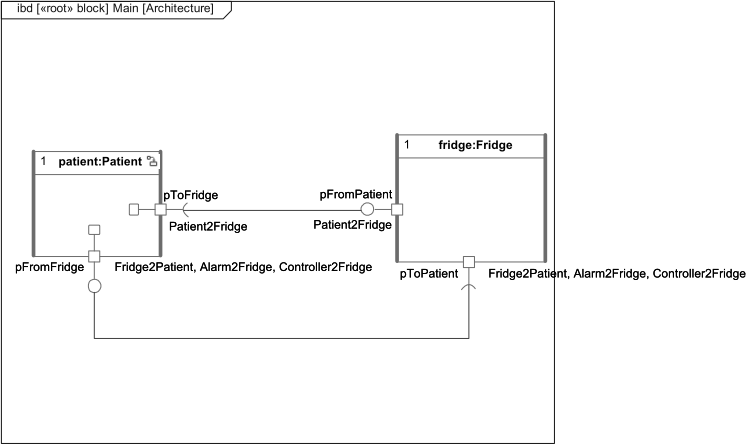
\epsfig{file =MainIBD, width = 5.5cm}}
  \caption{Main Internal Block Diagram}
  \label{fig:mainibd}
 \end{figure}

%Fig.~\ref{fig:aalblocks} shows the blocks with ports that we have identified in the AAL system. 

%\begin{figure}[!h]
%  \vspace{8cm}~
%  \centering
%  {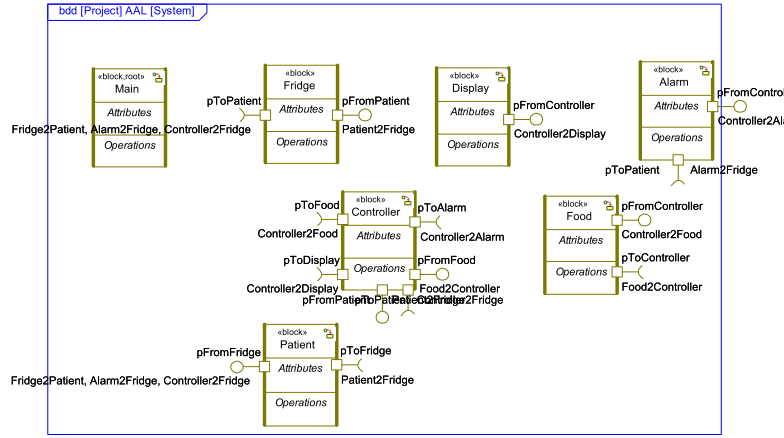
\epsfig{file =AALBlocks, width = 5.5cm}}
%  \caption{AAL System Blocks}
%  \label{fig:aalblocks}
% \end{figure}

The important part of the AAL system is the intelligent Fridge. The Fridge interacts with the AAL system. The Fridge in turn is composed of four blocks: information about the Food it contains, its Controller, the Display and the Alarm. Each of these blocks behaviors is modeled in a separate state machine diagram. Fig.~\ref{fig:fridgeibd} shows the internal block diagram for the Fridge block.

\begin{figure}[!h]
  \vspace{8cm}~
  \centering
  {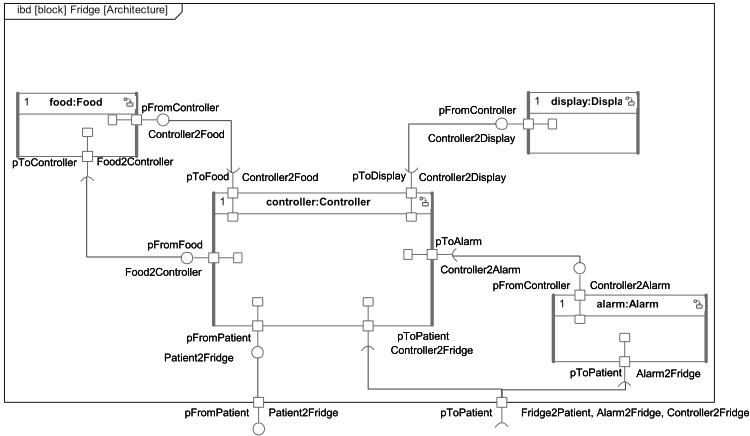
\epsfig{file =FridgeIBD, width = 5.5cm}}
  \caption{Fridge Internal Block Diagram}
  \label{fig:fridgeibd}
 \end{figure}


Fig.~\ref{fig:patientstm} shows the state machine diagram for the Patient block. Here the exchange of information between Patient and Fridge takes place. We identify the number and quantity of each time present in the Fridge. If a certain product still present in the Fridge is chosen by the Patient then the information is  communicated with the Fridge.  Otherwise the Fridge is empty and the Patient will wait to be refilled. Also, if the Alarm of the Fridge is raised due to  high intake of calories, the Patient stops eating and waits for the system to be unblocked.
 
\begin{figure}[!h]
  \vspace{8cm}~
  \centering
  {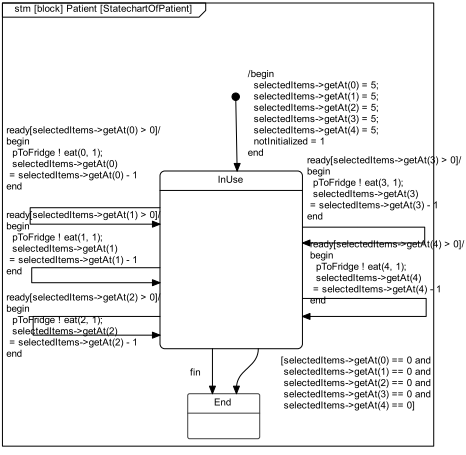
\epsfig{file =PatientSTM, width = 5.5cm}}
  \caption{Patient State Machine Diagram}
  \label{fig:patientstm}
 \end{figure}
 

The Food block models the knowledge of the Fridge about what it contains. Here we define the number of items and the amount of calories associated with each item present in the Fridge. We then calculate the total number of calories accumulated by the Patient. If the total number of calories is greater or equal to the maximum calories allowed for the Patient, then a message is send and the alarm is raised or if the total number of calories is greater than the maximum calories allowed minus 500, then the Patient is warned with a message that the calories level is approaching the maximum amount of calories allowed.

\section{\uppercase{Properties Verification of AAL system}}
\label{properties verification}
The properties of AAL system that we modeled and verified are obtained after \myrelax{} process is applied on its traditional requirements. \myrelax{}  is  a  requirement  engineering language for self-adaptive systems that incorporates uncertainty into the specification of these systems. Typical  textual  requirements  prescribe behavior  using  a  modal  verb  such  as  SHALL  that defines  functionality  that  a  software  system  must always provide. For self adaptive systems however, environmental  uncertainty  may  mean  that  it  is  not always  possible  to  achieve  all  of  those  SHALL statements; or behavioral uncertainty may allow for trade-offs between SHALL statements to \myrelax{} non-critical  statements  in  favor  of  other,  more  critical ones.  Therefore  \myrelax{}  identifies  two  types  of requirements:  one  that  can  be  \myrelax{}-ed  in  favor  of other ones called variant or \myrelax{}-ed and other that should never change called invariant.
Below are the properties to be verified: 
\subsection{Traditional/\myrelax{}-ed Requirement}

%\begin{description}
\begin{itemize}
\item The fridge shall detect and communicate with food packages
\end{itemize}
%\end{description}

\myrelax{}-ed version of this requirement is as follows:
%\begin{description}

\begin{itemize}
\item Property 1 : The fridge SHALL detect and communicate information with AS MANY food packages AS POSSIBLE
\end{itemize}

%\end{description}

Below are the uncertainty factors associated with the given \myrelax{}-ed requirement.

\begin{description}
\item[ENV:] Food locations, foot item information (type, calories), food state (spoiled and unspoiled)
\item[MON:] RFID readers, Cameras, Weight sensors
\item[REL:] RFID tags provide food locations and food information; Cameras provide food locations (Cameras provide images that can be analyzed to estimate food locations), Weight sensors provide food information (whether eaten or not)
\end{description}

\begin{figure}[!h]
  \vspace{8cm}~
  \centering
  {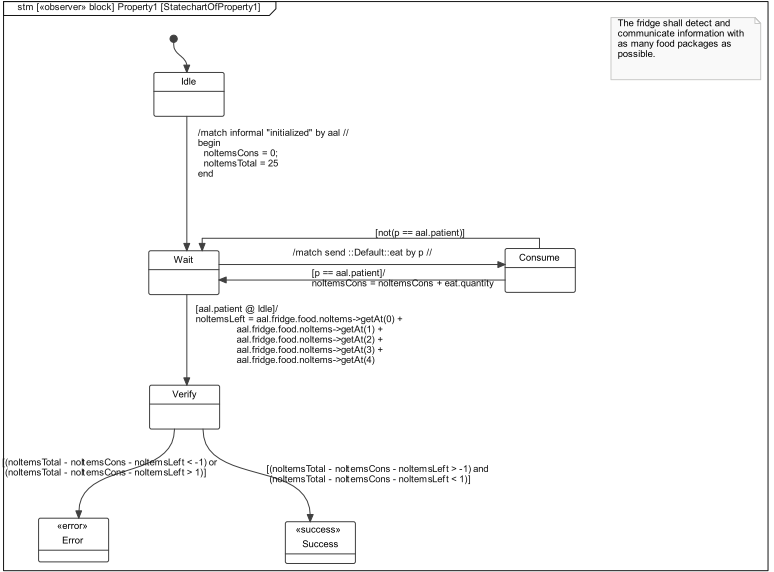
\epsfig{file =Property1STM, width = 5.5cm}}
  \caption{Property1 State Machine Diagram}
  \label{fig:property1stm}
 \end{figure}

The satisfaction of this requirement contributes to the balanced diet of the Patient. We would like to verify this property as it is important for the AAL system to know about as many food items as possible present in the fridge. 
Fig.~\ref{fig:property1stm} shows the state machine diagram of the Property 1. In this property, we identify the number of items consumed by the Patient and the total number of items in the Fridge. First of all, we verify the identity of the Patient, if the person is identified as the Patient, then we calculate the number of items consumed. We then calculate the number of items left in the Fridge which is equal to the sum of all the items present in the Fridge. Then in the last step, we calculate if the total number of items minus the number of items consumed minus the number of items left is greater than -1 and the total number of items minus the number of items consumed minus the number of items left is less than 1 i.e. it should be between -1 and 1 (there is no information loss). It means that we have reached the success state by having all the information about all the items present in the Fridge. Inversely, if the total number of items minus the number of items consumed minus the number of items left is less than -1 or the total number of items minus the number of items consumed minus the number of items left is greater than 1, then it means that we are missing some information about some of the items present in the Fridge and the observer passes into the error state.
Following are the two invariant requirements that we will verify.

\subsection{Invariant Requirement}

%\begin{description}

\begin{itemize}
\item Property 2 : The Alarm SHALL be raised instantaneously if the total number of calories surpasses the maximum calories allowed for the patient 
\end{itemize}


%\end{description}

\begin{figure}[!h]
  \vspace{8cm}~
  \centering
  {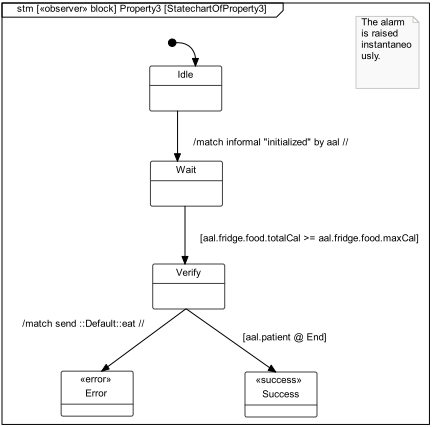
\epsfig{file =Property3STM, width = 5.5cm}}
  \caption{Property2 State Machine Diagram}
  \label{fig:property3stm}
 \end{figure}

This property ensures that the Patient should stop eating when the total number of calories surpasses the maximum calories allowed and that the alarm should be raised.
Fig.~\ref{fig:property3stm} shows the state machine diagram of the property 2. This requirement implies that the Alarm shall be immediately raised as soon as the total number of calories equals or surpasses the maximum calories allowed for the Patient. If it happens then the Patient should stop eating.  

\subsection{Verification Results}
Until now, we have modeled the AAL system and the properties to be verified on the model. Fig.~\ref{fig:xmi2if} shows the snapshot of the compilation of the AAL model named AAL2. The AAL2 model is first exported into AAL2.xmi and then using the IFx toolset the AAL2.xmi is compiled into AAL2.if.

\begin{figure}[!h]
  \vspace{8cm}~
  \centering
  {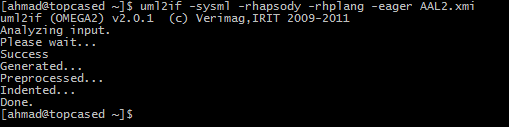
\epsfig{file =Xmi2If, width = 5.5cm}}
  \caption{XMI to IF Compilation}
  \label{fig:xmi2if}
 \end{figure}
 
\begin{figure}[!h]
  \vspace{8cm}~
  \centering
  {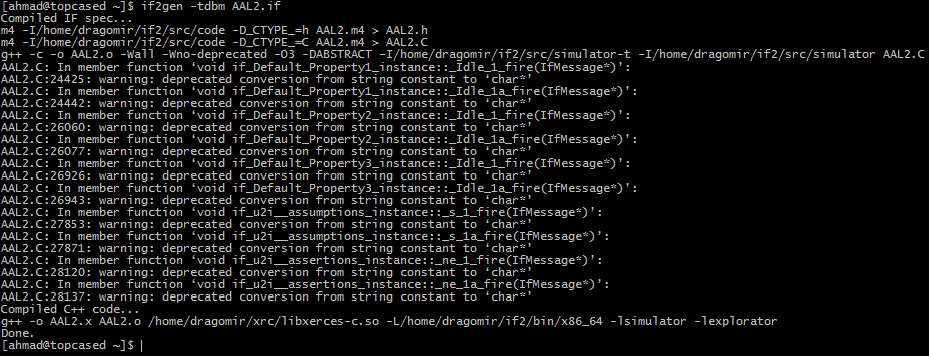
\epsfig{file =If2Exe, width = 5.5cm}}
  \caption{IF to Executable file Compilation}
  \label{fig:if2exe}
 \end{figure}

Fig.~\ref{fig:if2exe} shows the snapshot of the compilation of AAL2.if into an executable file i.e. AAL2.x. 
For the properties verification part, we run the model-checker with the following options:
AAL2.x -dfs -po -me -ce –ln
While verifying the AAL model, the model-checker has found several error scenarios, as one can see in Fig.~\ref{fig:errorstate}.  Any of the error scenario can then be loaded through the interactive simulation interface of the IFx toolset to trace back the error in the model and then correct it. 


\begin{figure}[!h]
  \vspace{8cm}~
  \centering
  {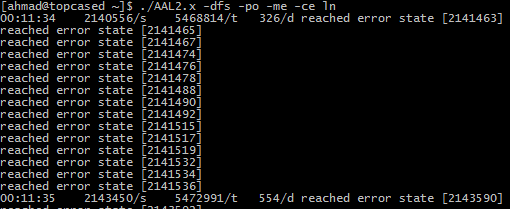
\epsfig{file =ErrorState, width = 5.5cm}}
  \caption{Model Checker results in Error Scenarios}
  \label{fig:errorstate}
 \end{figure}


In order to  debug  a model, firstly we import it into the simulator as shown in Fig.~\ref{fig:initialsimulationinterface} .

\begin{figure}[!h]
  \vspace{8cm}~
  \centering
  {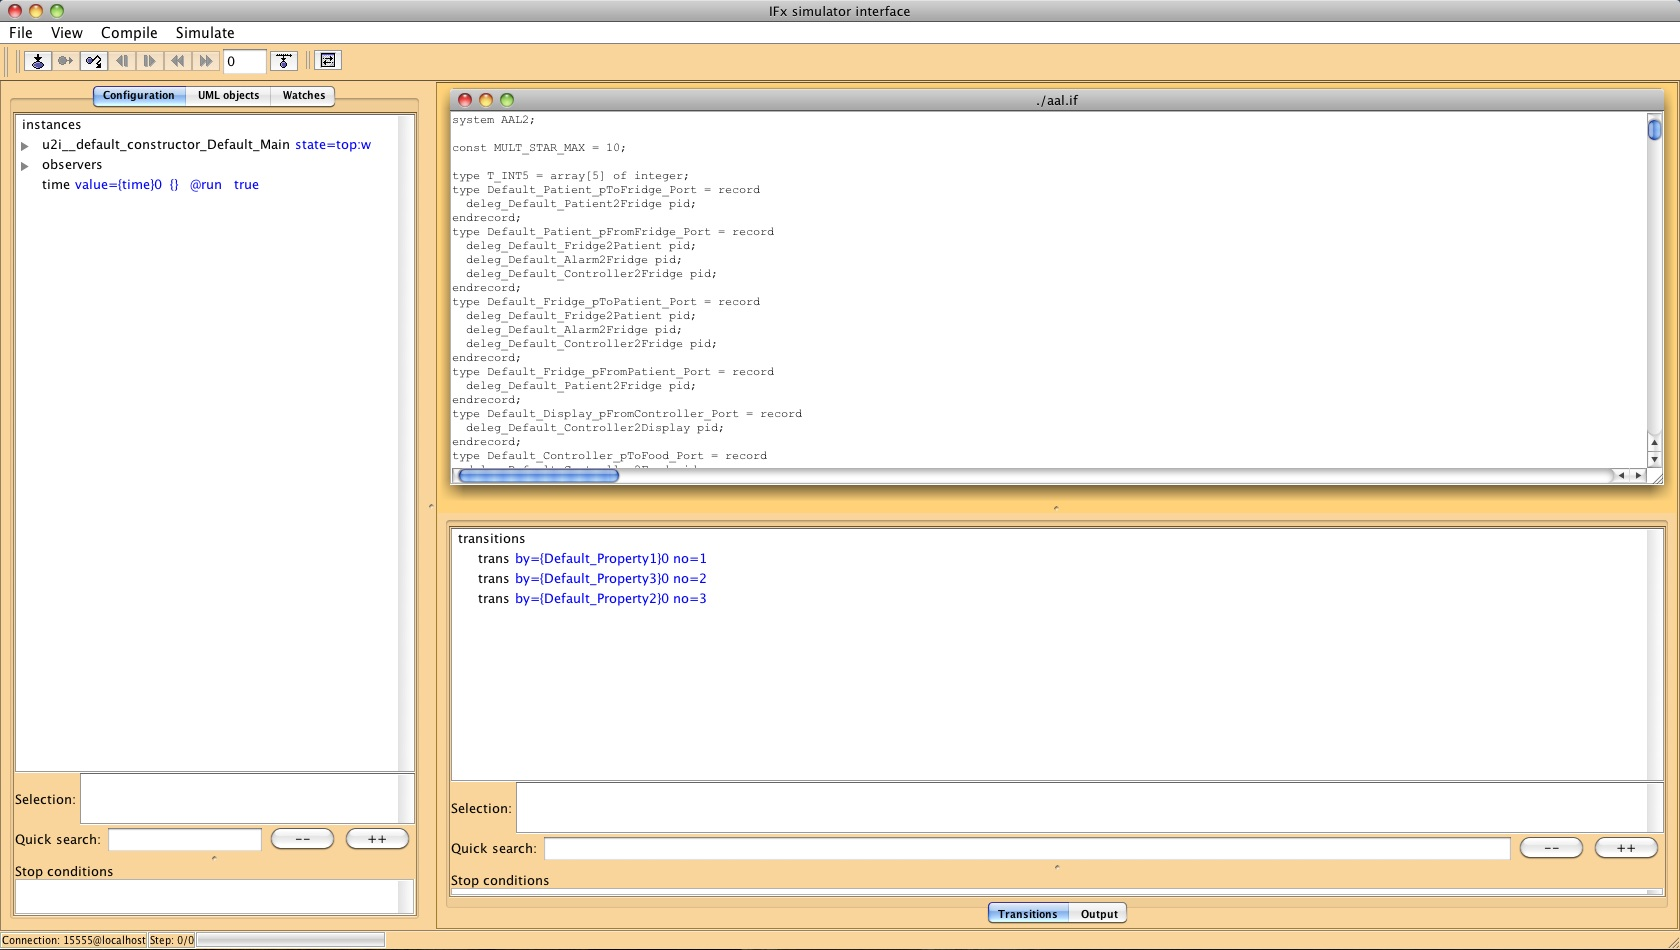
\epsfig{file =InitialSimulationInterface, width = 5.5cm}}
  \caption{Initial Simulation Interface}
  \label{fig:initialsimulationinterface}
 \end{figure}

We check the states of the \textit{observers} in order to identify which property has not been satisfied. One can observe in Fig.~\ref{fig:errorstatefoodobserver} that Property 3 fails. While checking the state of the entire system for this property, we discover that the error state contained the maximal allowed number of calories for the total number of calories consumed and subsequently eat requests sent by the Patient. This implies that the Alarm function of the intelligent Fridge doesn't function properly. The Alarm function of the Fridge is strictly relied to its Food process. 

%One can observe in the state machine of this block Fig.~\ref{fig:foodstm}  that 

The Alarm is raised only if the total number of consumed calories is strictly superior than the maximum allowed; condition which doesn't satisfy the request that the Alarm is raised as soon as possible. The correction consists in raising the Alarm in case the total number of consumed calories is equal to the maximum allowed threshold. Once this error is corrected the verification succeeds.

\begin{figure}[!h]
  \vspace{8cm}~
  \centering
  {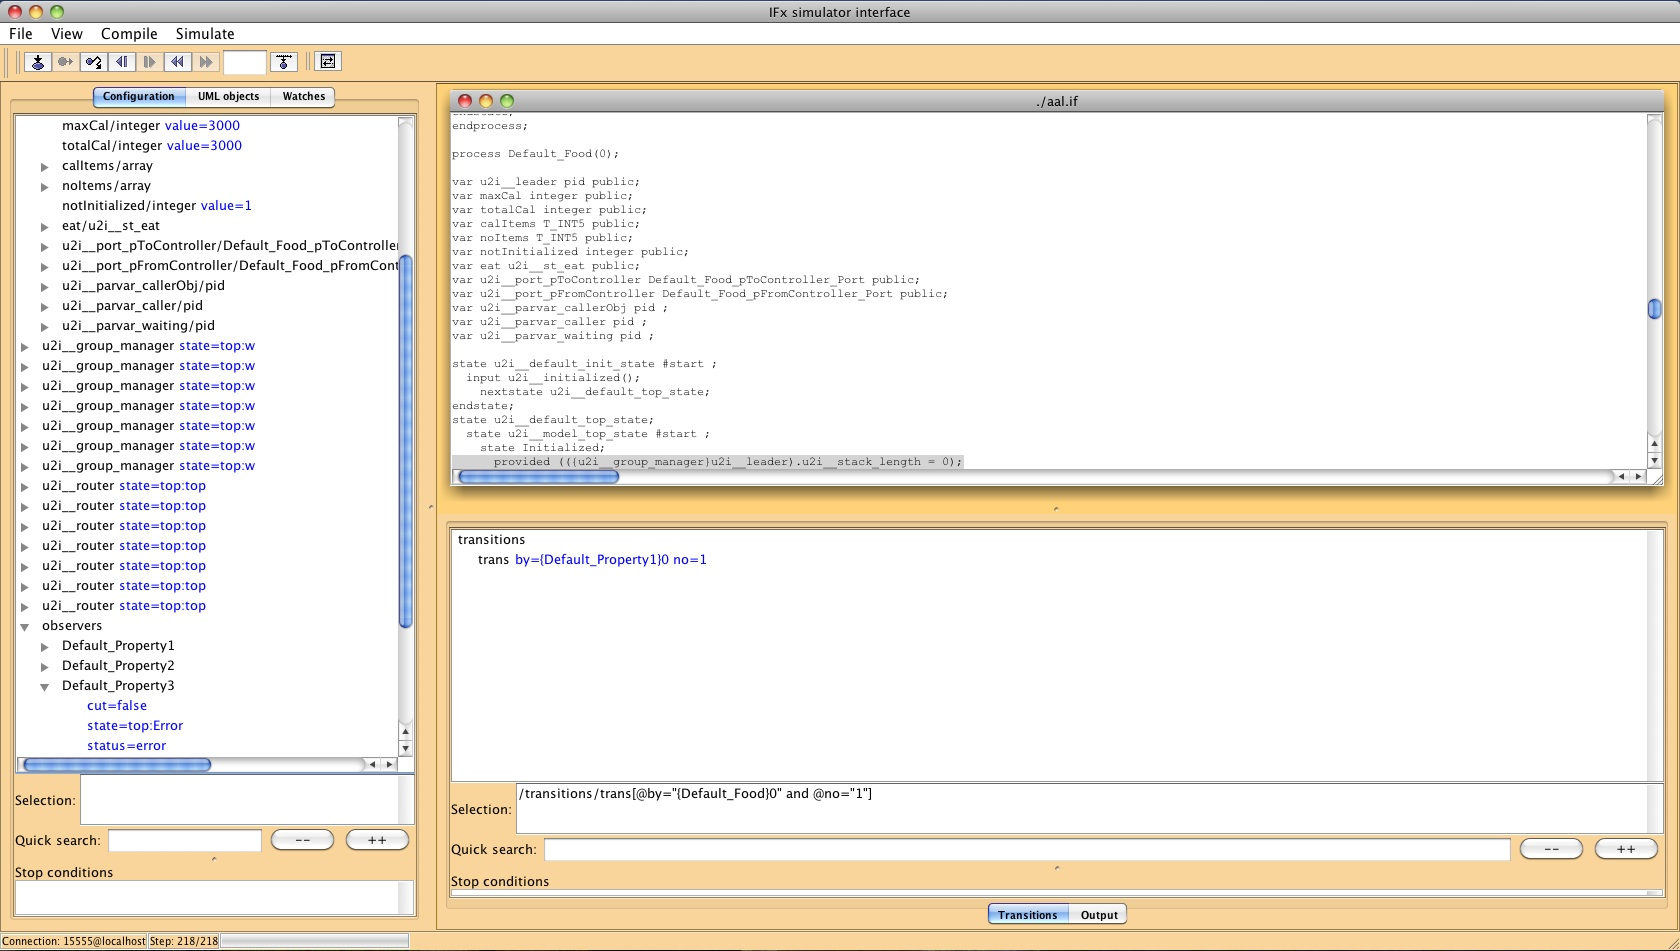
\epsfig{file =ErrorStateFoodObserver, width = 5.5cm}}
  \caption{Error State Food Observer Simulation Interface}
  \label{fig:errorstatefoodobserver}
 \end{figure}

\begin{figure}[!h]
  \vspace{8cm}~
  \centering
  {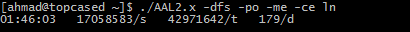
\epsfig{file =VerificationOk, width = 5.5cm}}
  \caption{Model checking successful}
  \label{fig:verificationok}
 \end{figure} 

Fig.~\ref{fig:verificationok} shows the result of the model-checker on the correct model.

\section{{Conclusion}\label{conclusion}}
We have modeled the structural and behavioral parts of an AAL (Ambient Assisted Living) system. The modeling is done using Rational Rhapsody 7.5.2  with OMEGA2 profile which is used for specification and verification of dynamic properties of models through \textit{observers}. For the verification and simulation part, we have used IFx which is a toolset used for the simulation of OMEGA2 models and the verification of properties defined on these models. We have verified two properties of the AAL system using the IFx toolset. In one case, the verification results in the fulfillment of all the two properties and in other case the verification results in errors which can then be simulated through the interactive simulation interface of the IFx toolset in order to identify the source of the error and then subsequently correct it in the model. 

The future work is centered around the use of observers in the context of our integrated approach \cite{test9}. This paper motivated us to take benefit from the OMEGA2/IFx. In our integrated approach, we are interested in \myrelax{} requirement which we obtain by using the \myrelax{} process. We then refine the \myrelax{} requirement with the ContributionType and ContributionNature of \sysml{}/\kaos{} \cite{test10} which is a \sysml{} profile with the goal concepts integrated into it. The \myrelax{} requirement is then verified by a test case and then the test case can be refined by observer and then observer is allocated to a state machine diagram. This whole sequence of steps constituit our meta model.
%The application of OMEGA2 profile to models is straight forward in that one only needs to add the predefined library provided with the tool (OMEGA2.sbs and OMEGA2Predefined.sbs) into the model. After the creation of OMEGA2 models, export to an xmi file is simply done through the Rational Rhapsody v7.5.2 menu. The choice of the version of Rational Rhapsody is very important as OMEGA2/IFx is not compliant with the new versions of Rational Rhapsody. Another important point to mention is the time the IFx toolset takes for the verification of properties as it depends on the number of items present in the Fridge i.e. in our case study, we have five items in the Fridge and the model checker took considerable amount of time to check all the states of the system. 

\bibliographystyle{apalike}
{\small
\bibliography{example}}

\begin{thebibliography}{1}

\bibitem{test1} 
http://www-2.cs.cmu.edu/~svc/

\bibitem{test2} Iulian Ober and Iulia Dragomir. OMEGA2: A new version of the profile and the tools, 15th IEEE International Conference on Engineering of Complex Computer Systems, DOI 10.1109/ICECCS.2010.59.

\bibitem{test3}  IBM, “Rational Rhapsody v7.5. reference manuals.” Available via http://www.ibm.com/developerworks/rational/.

\bibitem{test4}  Iulian Ober, Susanne Graf and Ileana Ober. Validating timed \uml{} models by simulation and verification, International Journal on Software Tools for Technology (2006) 8(2): 128–145 DOI 10.1007/s10009-005-0205-x

\bibitem{test5}E. M. Clarke, O. Grumberg, and D. A. Peled, Model Checking. MIT Press, 1999.

\bibitem{test6} Jon Whittle, Pete Sawyer, Nelly Bencomo, Betty H.C. Cheng, and Jean-Michel Bruel. \myrelax{} : Incorporating Uncertainty into the Specification of Self-Adaptive systems, Proceedings of the 17th IEEE International RE Conference, Pages: 79-88

\bibitem{test7} OMEGA-IFx for \uml{}/\sysml{} v2.0 Profile and Toolset, User Manual Document version 1.1

\bibitem{test8} https://wwwsecu.irit.fr/
FILEX/get?k=n21pV3UgsOtvJC4PSvx

\bibitem{test9} Jean-Michel Bruel, Nicolas Belloir and Manzoor Ahmad. SPAS: un profil \sysml{} pour les syst`emes auto-adaptatifs, In 15`eme Colloque National de la Recherche en IUT (CN-RIUT), Lille, June 8th to June 9th, 2009.

\bibitem{test10} Christophe Gnaho, Farida Semmak. Une extension \sysml{} pour l’ing´enierie des exigences non-fonctionnelles orient´ee but, Revue Ing´enierie des Syst`emes d’Information, Vol 16 / 1, 23 pages, 2011.

\bibitem{BornotS00}
S.~Bornot and J.~Sifakis, ``{An algebraic framework for urgency},''
  \emph{Information and Computation}, vol. 163, 2000.

\bibitem{BozgaGOOS04}
M.~Bozga, S.~Graf, I.~Ober, I.~Ober, and J.~Sifakis, ``{The IF Toolset},'' in
  \emph{Formal Methods for the Design of Real-Time Systems}, ser. Lecture Notes
  in Computer Science, M.~Bernardo and F.~Corradini, Eds.\hskip 1em plus 0.5em
  minus 0.4em\relax Springer Berlin / Heidelberg, 2004, vol. 3185, pp.
  131--132.

\bibitem{OberD11}
 I.~Ober and I.~Dragomir, ``{Unambiguous UML Composite Structures: The OMEGA2 Experience},'' in
  \emph{SOFSEM 2011: Theory and Practice of Computer Science}, ser. Lecture
  Notes in Computer Science, I.~Cerna, T.~Gyimothy, J.~Hromkovic, K.~Jefferey,
  R.~Kralovic, M.~Vukolic, and S.~Wolf, Eds.\hskip 1em plus 0.5em minus
  0.4em\relax Springer Berlin / Heidelberg, 2011, vol. 6543, pp. 418--430.

\end{thebibliography}
%\section*{\uppercase{Appendix}}
%
%\noindent If any, the appendix should appear directly after the
%references without numbering, and not on a new page. To do so please use the %following command:
%\textit{$\backslash$section*\{APPENDIX\}}

\vfill
\end{document}

